\documentclass[12pt,journal,compsoc]{IEEEtran}

\usepackage[portuguese]{babel}
\usepackage[utf8]{inputenc}
\usepackage{graphicx}
\usepackage[font=small,labelfont=bf]{caption}
\usepackage{breakurl}
\usepackage{color}

\newcommand{\hilight}[1]{\textbf{\textcolor{red}{#1}}} % para ajudar a destacar TODOs e outros alertas

\begin{document}

\title{Carros elétricos para um mundo melhor}
\author{
  Daniel~M.~Assis, 
  Lindomar~G.~Ferreira, 
  Rodrigo~Magalhães
  \IEEEcompsocitemizethanks{
    \IEEEcompsocthanksitem D. M. Assis, L. Ferreira e R. Magalhães são mestrandos do Instituto de Pesquisas Tecnológicas do Estado de São Paulo
  }
}

\IEEEcompsoctitleabstractindextext{%
\begin{abstract}
Nos dias atuais, o software está envolvido em todas as atividades, de processadores de texto a operações de naves espaciais. Num cenário onde os aplicativos apoiam praticamente todas as atividades humanas, é esperado que haja muita demanda de software em uma das indústrias mais tradicionais: a automobilística. Associada a outra preocupação constante - o impacto no meio-ambiente -, este trabalho apresenta uma proposta para adição de valor, por meio de tecnologias de software, à seção de carros elétricos da empresa automobilística fictícia MotorBRAS. Expõe-se uma forma de aplicação de técnicas de engenharia de software que visam a geração de tecnologia para apoio à evolução do negócio, por meio de organização de um setor de desenvolvimento de software que aplique as devidas técnicas.  
\end{abstract}
\begin{IEEEkeywords}
Engenharia de Software, SWEBOK, Scrum
\end{IEEEkeywords}}

\maketitle

\IEEEdisplaynotcompsoctitleabstractindextext
\IEEEpeerreviewmaketitle


\section{Introdução ao Projeto}

\IEEEPARstart{N}{os} dias atuais, poucas coisas são mais importantes para a Humanidade quanto a questão da ecologia. Na proporção em que crescemos enquanto espécie, a projeção média de crescimento da população mundial é de 9 bilhões de pessoas até 2050. \cite{wwf_living_2013} Esse crescimento populacional influi diretamente nas condições de vida no planeta.

Desta forma, no que concerne à área de atuação da MotorBRAS, a redução no controle de emissões de gás carbônico apresenta-se, mais do que nunca, como um diferencial competitivo atraente. Países mais desenvolvidos estão prontos e dispostos a investir em tecnologias para redução do consumo de CO2, de forma que o risco no investimento em tecnologias ambientais apresenta-se como baixo, uma vez que a demanda por novas tecnologias neste campo é cada vez mais atrativa. As empresas que forem pioneiras no investimento de tecnologias ambientais que influenciem a vida das pessoas terão uma ótima vantagem competitiva em relação aos concorrentes. 

Este projeto visa agregar valor à intenção da MoToRBRAS de entrar no mercado de carros elétricos como serviço até 2020. A proposta é a de agregar tecnologia ao produto, de forma a cativar o consumidor em relação ao serviço e, assim, mitigar o impacto do Homem no meio ambiente. Consequências diretas são a geração de uma imagem positiva no mercado, bem como a conquista de uma posição de vanguarda e liderança no mercado. 

Países desenvolvidos são favoráveis à ideia de aluguel de carros elétricos em suas grandes cidades, como forma de locomoção barata e rápida das pessoas para seu local de trabalho. Carros elétricos, sendo pequenos e de baixo consumo, são altamente atrativos como um meio-termo entre os carros particulares e o transporte público. 

O que este projeto propõe é tornar esse serviço ainda mais atrativo, através da customização de cada carro, pelo uso de tecnologia de ponta. O diferencial é permitir que o carro seja automaticamente customizado para o indivíduo. 


\section{Condições e Características Importantes}

De acordo com o projeto previsto pelo grupo, as seguintes características serão agregadas aos carros elétricos:

\begin{itemize}

\item Reconhecimento de íris: uma maneira eficaz de identificar o indivíduo para então iniciar o processo de customização de suas preferências;

\item Integração com redes sociais: para que seja possível ao indivíduo ter acesso a sua agenda, contatos, calendários e preferências musicais instantaneamente; 

\item Customizações físicas internas: preferências como temperatura do carro (ajuste do ar condicionado) e posição do banco serão carregadas de um servidor central e aplicadas diretamente ao veículo quando da identificação do indivíduo; da mesma forma, alterações no veículo são salvas no servidor central como preferências do indivíduo, para posterior aplicação numa nova viagem;

\end{itemize}

Além das características acima citadas, outros aspectos devem ser considerados para garantir o correto funcionamento de todo o processo, tais como:

\begin{itemize}

\item Segurança: um aspecto importante que deve ser considerado em todo o projeto, tanto pelo aspecto de segurança da identidade do indivíduo quanto pela segurança na execução das tecnologias físicas de customização e carregamento automático, bem como pela segurança nas transações de aluguel do veículo;

\item Controle cadastral: o gerenciamento da customização das preferências e do pagamento pelo serviço são aspectos que também devem ser endereçados, de forma que um sistema para controle cadastral dos clientes faz-se necessário.

\end{itemize}

Além dos sistemas internos ao veículo, são necessários softwares externos para compor a infraestrutura de prestação de serviços. Esses softwares são:

\begin{itemize}

\item Sistema para aluguel de veículos pelos cliente:componente importante da infraestrutura de prestação do serviço, este software permitirá que os motoristas interessados efetuem agendamento e posterior pagamento pelo serviço de aluguel de veículo através da internet;

\item Sistema para gestão da frota de veículos: o processo de gestão da frota de veículos requer um software de apoio. Atividades de manutenção, abastecimento, disponibilização e recepção de veículos nos pátios, entre outras, serão suportadas por esse software. Este software representará o elo entre o processo de aluguel de veículos e as atividades administrativas e operacionais ligadas à gestão da frota.

\item Servidor de armazenamento de perfis: software executado em um servidor centralizado que armazenará as preferências de cada usuário, bem como efetuará, de forma segura, a ponte entre o veículo e os dados disponíveis nas redes sociais do motorista.

\end{itemize}

Algumas características do produto e do contexto de negócios influenciarão a formatação do projeto. A listagem de características e respectivas consequências para o projeto são:

\begin{itemize}

\item Alto nível de inovação do produto: não existem serviços similares no mercado brasileiro. Estamos tomando como base a experiência de serviços semelhantes em outros países, mas, devido a fatores culturais, existe a possibilidade da experiência não se repetir com sucesso em nosso mercado. Tal situação possivelmente levará a uma proposta de adaptação pelo departamento de marketing, o que, por sua vez, exigirá a capacidade de absorção de novos requisitos por parte da TI. Dessa forma, optamos pela adoção de métodos ágeis, que são mais adequados a esse tipo de ambiente de negócio.

\item Heterogeneidade dos softwares a serem desenvolvidos: diferentes tipos de software serão desenvolvidos - desde sistemas desktop administrativos, passando por softwares para servidores e chegando a software embarcado para execução dentro do veículo. Esse contexto torna interessante a ideia da criação de pequenas equipes, especializadas no domínio específico da aplicação que estão desenvolvendo, dedicadas à atuação apenas no software que atende suas respectivas especialidades.

\end{itemize}

\section{Disciplinas do SWEBOK}

As disciplinas do SWEBOK serão aplicadas pelos times de desenvolvimento conforme segue: 

\subsection{Requisitos}

Os requisitos de produto serão expressos por meio de uma especificação composta
de histórias \cite{primo_user_2011}, por ordem de prioridade, que são definições funcionais de alto
nível. O analista de requisitos será responsável por prover informações
detalhadas referentes às histórias aos demais membros do time, no momento de
estimativa da iteração e durante toda a iteração. Desta forma, cabe a este
profissional ter o entendimento dos detalhes das histórias. Será entregue, a
cada iteração, uma documentação que detalha os aspectos importantes de cada
história realizada. 

Um engenheiro de software com perfil mais técnico também precisará ser envolvido no entendimento dos requisitos juntamente com o analista de requisitos, pois a visão técnica que considera os requisitos não-funcionais deve ser analisada ao mesmo tempo em que os requisitos surgem.

O tester também deve estar no levantamento de requisitos, para prover uma visão mais funcional que permita que a definição da especificação seja definida de uma forma funcional e testável.

Os analistas de requisitos precisarão ter livre acesso aos stakeholders (pessoal
de marketing e parte jurídica, que atuam como reguladores), que vão fornecer e
auxiliar na validação dos requisitos. Esse acesso deverá ser feito através de
entrevistas, onde podem-se fazer uso de protótipos pela técnica de DDD \cite{evans_domain-driven_2004}  
(mais do que o rigor do UML) e exemplificação de
cenários como formas de obter clareza nos detalhes das histórias. Os modelos
conceituais estão a cargo dos entrevistadores, e não definem característica
formal. Apenas é esperado que sejam definidos cenários para cada história
\cite{washington2003using}, de forma a guiar o time durante a construção e
permitir geração de validação automatizada dos requisitos
\cite{melnik_multiple_2007}.

Considerando a característica dinâmica da equipe de marketing, assume-se que os requisitos são voláteis; a abordagem para mudanças é a de tentar incorporar o máximo possível se a história permanecer a mesma, mas caso trate-se de outra história, incorporar apenas na próxima iteração, como forma de não impactar os prazos e custos do projeto \cite{zowghi2002study}.

Uma arquitetura será definida com base no entendimento das primeiras histórias da especificação (e com base em conhecimento da visão geral do projeto e características de infra-estrutura da empresa), e evoluída durante todo o projeto \cite{cohn_agile_2009}, apoiando-se em técnicas como refatoração e automatização de testes de regressão.

Os requisitos serão validados através de testes de aceitação, de duas formas:
manual (na reunião de demonstração da iteração, quando os stakeholders comparam
as histórias combinadas em relação ao funcionamento do sistema), e
automatizada: utilizando a técnica de BDD \cite{chelimsky2010rspec}, cada
cenário de cada história será vinculado a métodos de teste durante a
construção, de forma que cada execução da suite de testes irá gerar um
relatório que define se as histórias estão funcionando de acordo com o
esperado.

\subsection{Design}

No início do projeto (antes da primeira iteração), considerando a visão geral e o entendimento dos requisitos de maior prioridade, o design de software arquitetural (top-level) será definido por um engenheiro de software com perfil sênior em desenvolvimento. Após isto, a cada iteração, o trabalho de design detalhado será incorporado no trabalho dos desenvolvedores da equipe, de forma que o design não será mais dissociado da construção, e sim será parte desta \cite{fowler_planned_evolutionary_design}. O engenheiro sênior em desenvolvimento pode definir design arquitetural para futuras iterações, dependendo da necessidade, e trabalhar juntamente com o time na definição do design detalhado, durante a iteração. O design arquitetural deverá ser documentado em alto nível, considerando aspectos como estilo arquitetural sendo utilizado, forma de tratamento de eventos, forma de lidar com concorrência, distribuição de componentes, persistência de dados.

Já a responsabilidade de design detalhado cabe a todos os desenvolvedores do time, e não será exigida documentação formal para tal, pois assume-se o conceito de que o "código-fonte é o design" (ou seja, seguindo a visão de design do XP, o design existe como uma forma diferente, significando a prática de manter o código claro, uso de práticas de refatoração, conhecimento e aplicação de padrões de projeto, ter um olho em mudanças futuras e saber comunicar o design por meio de conversação \cite{fowler_design_dead}). Contudo, será necessário validar a qualidade deste design, o que será feito através da elaboração de relatório de inspeção de código a cada iteração, que deve considerar as questões do documento de design arquitetural, além de técnicas de design, como: abstração, acoplamento, coesão, decomposição, modularização, encapsulamento, separação de responsabilidades, design patterns. 

O relatório será realizado pelo engenheiro de software da própria equipe que agregar o papel de sênior, e deve ser entregue como um artefato da iteração (relatório de qualidade de design). A responsabilidade pela veracidade do documento é de toda a equipe.

Além deste relatório, a qualidade do design também será garantida através de:
\begin{itemize}
\item práticas diárias de DDD: para permitir uma modelagem do design alinhada com as regras de negócio sendo utilizadas. O DDD faz uso de um diagrama simplificado de classes para modelar o entendimento;
\item práticas diárias de pair programming e TDD \cite{begel_pair_2008}\cite{nagappan_realizing_2008}: que orientam o desenvolvedor no sentido de escrever um código claro e seguindo o paradigma de orientação a objetos;
\item práticas automatizadas: análise estática de código, para garantir que boas práticas de design estão sendo adotadas no código sendo escrito \cite{karpov_static_code_analysis}. Esta prática não deve ser avaliada apenas no final da iteração, mas diariamente, por todo o time.
\end{itemize}

Em relação às descrições estruturais, espera-se que o documento de arquitetura defina diagramas de deployment, e é desejável que os diagramas de classes simplificados que surgem da prática de DDD também sejam documentados (a ser definido pelo time).

Para este projeto, a estratégia de design é baseada em design orientado a objeto, por ser um modelo comumente difundido pelos membros do time e por ser adequar ao projeto proposto.


\subsection{Construção}

Este projeto tratará design e construção de forma muito próxima. Os engenheiros de software com perfil de programadores terão poder de definir o design detalhado bem como a codificação, sempre orientados por um programador sênior e pelo design arquitetural. O programador poderá, portanto, aplicar os fundamentos de minimização de complexidade, antecipação de mudanças e construção para verificação tanto em design quanto em construção, sem a necessidade de haver distinções.

É esperado que o programador reduza a complexidade em tudo o que for fazer, utilizando os melhores algoritmos e padrões. Também é esperado que o código seja escrito de forma a permitir futuras modificações sem grande impacto (e para isso, é exigido que a prática de TDD seja adotada, e o conceito de refatoração seja entendido \cite{Fowler1999}). Outras práticas que serão exigidas do programador são a escrita de testes unitários e de integração \cite{unit_int_func_testing}. A verificação da adoção destas práticas será realizada juntamente com a validação de qualidade do design, descrita no tópico anterior. 

Também será exigido que o programador escreva testes de aceitação baseados em BDD \cite{chelimsky2010rspec}, contra cada história da especificação que implementa, para garantir que seu código seja verificável. Estes testes serão executados diariamente, gerando relatórios que indicam se o código é válido em relação ao esperado. Será exigido que o programador siga os padrões de desenvolvimento de código da empresa, e a ferramenta de análise estática de código irá indicar se os padrões estão sendo ignorados, diariamente, durante a iteração. Códigos não-conformes devem ser corrigidos o mais rápido possível, no prazo máximo de duração da iteração.

Não será exigido uso formal de UML; contudo, o time pode optar por utilizar UML (bem como qualquer outra forma visual de design) para facilitar a comunicação e/ou o entendimento de um dado objeto ou conjunto de objetos que precisa ser criado ou alterado. 

O modelo de construção que será adotado neste projeto é o Scrum
\cite{schwaber_scrum_2013}. Este modelo iterativo trata a construção de forma
concorrente a outras atividades de desenvolvimento de software, como os
requisitos, o design e os testes. Todas estas atividades interagem juntamente
nesta fase de construção; desta forma, o planejamento da construção se dá
iterativamente, envolvendo todas as atividades: desde a fase de análise (com a
definição dos requisitos da especificação como histórias por ordem de
prioridade, e o entendimento profundo destas através da elaboração de
cenários), passando por  uma estimativa para a iteração (onde time discute e
define quantas histórias da especificação podem ser realizadas, considerando a
prioridade) e pela construção propriamente dita (onde os programadores geram
código considerando design, os analistas documentam as histórias e os testers
validam as histórias contra o sistema conforme vão sendo finalizadas), e
finalizando na entrega (onde os stakeholder validam, numa reunião de
demonstração, o sistema rodando, a documentação e demais artefatos que tenham
sido previamente combinados a serem entregues).  Para medida das iterações, são
utilizadas as métricas já descritas nos tópicos anteriores, bem como o próprio
aval dos stakeholders.


\subsection{Testes}

A verificação dinâmica dos testes será aplicada pelo engenheiro de software com perfil de tester durante cada iteração, assim que uma data história for dada como pronta pelos engenheiros de software com perfil de programadores. Para este fim, os programadores devem liberar cada história pronta num servidor de testes.

A verificação, num primeiro momento, deve contemplar o conjunto de cenários da
história (teste de conformidade, ou teste funcional) e a análise dos relatórios
automatizados gerados pelo framework de BDD \cite{chelimsky2010rspec}.

Como já dito, o tester deve participar na fase de levantamento de requisitos, para auxiliar o analista na definição das histórias e cenários específicos; neste ponto, em sua área de conhecimento, garante critérios de seleção e adequação dos testes, bem como o objetivo e a efetividade dos testes. O ganho adicional com qualidade vem do fato de considerar que os programadores escrevem a aplicação partindo da mesma ótica, o que auxilia na redução de falhas de comunicação e de entendimento.

Deseja-se que o tester tenha perfil multidisciplinar o suficiente para que
possa atuar nos diferentes Níveis de Teste previstos em
\cite{society_software_2004}, sendo eles: os Testes Unitários, os Testes de
Integração e os Testes de Sistema. Considerando o emprego da técnica de pair
programming, o tester poderá até mesmo auxiliar os programadores nesta
atividade.  Contudo, esta atividade não é obrigatória, sendo esperado que o
foco do tester mais voltado ao aspecto funcional do software. 

No que concerne aos Testes de Sistema, o tester se concentrará em diversos
requisitos não-funcionais, verificando se eles estão de acordo com o esperado
(com o apoio do documento de design arquitetural e dos programadores), além de
analisar aspectos como performance, stress, configuração, usabilidade.
Espera-se que faça uso de  ferramentas para automatizar tais testes, e que gere
um relatório no final de cada iteração, referente a estes testes específicos.

Os testes de regressão funcionais devem ser automatizados, cobrindo os aspectos funcionais de maior importância (a serem definidos pelo próprio tester). Os aspectos não-funcionais não são esperados em relação à regressão, pois sua característica não sugere regressão, mas sim diagnóstico pontual.

O tester tem liberdade para decidir realizar testes estruturais, testes exploratórios e demais técnicas de testes que julgar válidas na iteração. Estes testes também precisam ser documentados em relatório, com justificativa e resultados. Os testes precisam ser planejados no início da iteração, e tal definição precisa também constar no relatório a ser entregue no final da iteração.


\subsection{Manutenção}

A equipe que dará manutenção é a mesma que desenvolveu o produto \cite{fowler_products_not_projects}. Desta forma,
qualquer nova requisição de modificação (evolução ou correção) deve ser
definida na especificação, seja alterando ou adicionando novos itens. Tal item,
então, precisa ser definido em forma de história e com prioridade, para
ingressar numa próxima iteração, seguindo o mesmo fluxo de um novo requisito.
Desta forma, incorporando correções no fluxo normal de desenvolvimento (e não
após todo o projeto ter terminado), procura-se eliminar o problema onde 80 por
cento do esforço de manutenção é gasto em ações não corretivas. Neste caso, a
manutenção acontece enquanto o projeto ainda existe, e a prioridade fica a
cargo dos stakeholders \cite{schwaber_scrum_2013}. 

A evolução do software, portanto, será agregada durante o projeto de desenvolvimento, cabendo apenas que haja um gerenciamento dos requisitos em relação à prioridade. Como a equipe é a mesma, não há transição de conhecimento. As manutenções corretivas, adaptativas e perfectivas irão entrar no fluxo normal de desenvolvimento. Já espera-se que a manutenção preventiva seja um trabalho implícito, resultante das práticas de qualidade e métricas nas fases de análise, design e construção. No caso especial da construção, espera-se aplicação de refatoração e code review.

A definição de testes de regressão de outras fases também irá ajudar na manutenção, definindo aspectos que não funcionam mais conforme esperado. Os testes de aceitação automatizados com BDD também garantem a mesma regressão, mas num nível mais alto: que as funcionalidades continuam válidas. 

Espera-se que toda a qualidade definida até o momento (com testes automatizados, métricas e inspeção de design e análise) permitam que uma análise de impacto gere sempre um baixo custo, e que haja uma alta capacidade de manutenibilidade. 

Após a finalização do projeto, uma equipe menor será designada para manter o mesmo seguindo os mesmos princípios definidos até então, e com boa parte do mesmo pessoal, de forma a facilitar a transmissão de conhecimento. Esta futura equipe, poderá fazer uso dos documentos de especificação e design de arquitetura e das documentações de testes para entender o sistema de um aspecto funcional, e deverá estudar o código para entender um design mais detalhado. O esforço em qualidade é pago aqui, pois o código deve estar escrito de forma que seja fácil de entender e evoluir, de forma que a prática de engenharia reversa deve ser desconsiderada. 

Revisões e auditorias \cite{society_software_2004} deverão ser conduzidas
regularmente ao longo do ciclo de vida do produto (e não somente durante a
duração do projeto), de forma que desvios possam ser identificados e corrigidos
antes que causem maiores danos.

\subsection{Gerenciamento de Configuração}

As atividades de Gerenciamento de Configuração estão relacionadas com todas
as demais atividades \cite{society_software_2004}. Por conta disso, a gerência
responsável pela gestão do projeto e, posteriomente, do produto, deverá
garantir o estabelecimento e manutenção de todos os canais de comunicação
necessários.

Haverá uma gerência de configuração responsável pelo armazenamento de todos os
artefatos gerados nas fases de requisitos, design, construção, testes e
manutenção, bem como ferramentas necessárias a todas as áreas. O planejamento
desta gerência deve considerar apenas elementos de software, descartando
hardware e firmware por não serem aspectos cujo controle faz-se necessário. Não
caberá à gerência de configuração definir regras sobre os artefatos gerados
(com exceção do código-fonte gerado), de forma que os times podem versionar
livremente; contudo, precisa prover mecanismos para auditar a informação
(entende-se que estes mecanismos devem ser manuais, pela diversidade de
artefatos que um dado time pode produzir). 

Em relação ao código-fonte gerado, a gerência de configuração precisará garantir sua qualidade através da análise estática de código com uso de ferramenta automatizada, de forma a garantir que o código está seguindo as boas práticas determinadas pela empresa. Relatórios desta medida de qualidade de código devem estar disponível para consulta a qualquer momento. O desenvolvedor deve possuir acesso a estas mesmas práticas, de forma a poder criar um código-fonte de acordo com as práticas exigidas pela gerência de configuração. 

Outra característica que precisa ser considerada é a permissão de acesso. Apenas usuários de um dado projeto podem ter permissão de acesso ao repositório de informações do projeto, a não ser que a gerência diga o contrário. Assim sendo, é preciso haver uma forma automática de conceder acessos, tanto individuais quanto a grupos, de forma que um privilégio individual de um elemento num grupo possa sobrescrever seu privilégio enquanto membro do grupo.

Esta gerência também será responsável pela integração contínua
\cite{fowler_ci_2006}: deverá prover e manter uma ferramenta de geração de
builds automatizados, a ser executada diariamente ("integrando" o código,
agregando a execução de testes unitários e de integração gerados pelos
programadores ao processo de build, gerando relatórios de métrica de cobertura
de testes, e notificando todo o time no caso de builds e testes quebrados), bem
como prover uma opção para geração de releases e deploy automático em servidor
de testes (base da entrega contínua). Estes relatórios poderão alimentar os
processos de Gerenciamento da Qualidade \cite{society_software_2004} e, além
disto, espera-se agilidade na entrega do sistema para validação pelos
stakeholders. 

Portanto, é responsabilidade da gerência de configuração gerar os releases/baselines. As baselines devem ser geradas a cada fim de iteração e os releases devem estar disponíveis para ser gerados sempre que a equipe de construção finalizar uma iteração, de forma que o ciclo de execução de trabalho deve estar alinhado com o desta equipe. Se o código-fonte não estiver conforme o validado pela análise estática de código e de acordo com as métricas de cobertura de testes geradas pela integração contínua, o release não poderá ser entregue. Cabe ao gerente de configuração a responsabilidade de alertar o time, de forma a evitar atrasos num entendimento tardio de que o release não poderá ser entregue por falta de qualidade.


\subsection{Gerenciamento de Engenharia de Software}

Ainda que seja considerado possível gerenciar software como qualquer outro processo complexo, este projeto considerará algumas especificidades de software \cite{society_software_2004}, tais como: 

\begin{itemize}
\item software deve ser construído como um processo iterativo, e não uma sequência de tarefas fechadas;
\item engenharia de software incorpora aspectos de criatividade e disciplina;
\item o grau de complexidade de software é alto;
\item existe uma rápida taxa de mudança em tecnologias envolvidas. 
\end{itemize}

Considerando tais especificidades, serão estabelecidas políticas de contratação de pessoal que valorizem profissionais atuantes e experientes em processos iterativos, e com conhecimento prático de tecnologias bem difundidas no mercado. O processo de desenvolvimento Scrum será utilizado por conta de ser um processo iterativo difundido \cite{scrum_development_process}. Em relação à plataforma de desenvolvimento, utilizaremos Java, pois além de ser uma das plataformas mais utilizadas no mundo há quase 20 anos \cite{tiobe_language} (provendo grande quantidade de recursos no mercado, além de bibliotecas, frameworks e documentação), seu escopo cobre tanto softwares Web quanto softwares embarcados (por meio do Android) - o que está diretamente vinculado à necessidade do projeto de rodar software tanto num servidor central quanto em cada carro, individualmente.

Uma vez que as pessoas certas tenham sido contratadas, deve-se verificar quais outros aspectos, como infraestrutura, suporte e expertise, também sejam  garantidos, de forma a validar a análise de viabilidade do projeto, garantindo, assim, que o projeto possa ser completado com sucesso de forma efetiva em prazo e custo \cite{society_software_2004}. Em relação às definições dos stackholders, durante todo o projeto será assumido que os requisitos e o escopo serão flexíveis, de forma a dar suporte à necessidade de alterações de ideias que o setor de marketing da MotorBRAS geralmente apresenta. Para dar suporte a estas alterações, e considerando que o Scrum será adotado, as mesmas serão realizadas diretamente no Backlog do produto, de forma a serem consideradas em iterações futuras, sem impactar a iteração corrente. \cite{schwaber_scrum_2013}

A associação de recursos com tarefas será realizada através da prática de User Stories: a criação de histórias que descrevem a necessidade do stackholder, e sua decomposição em tarefas e a associação de tarefas com recursos, é feita no planejamento de cada iteração. O conceito de User Stories não faz parte do Scrum, mas é comumente adotado em métodos ágeis como forma de orientar o trabalho a ser realizado na iteração \cite{user_stories_applied} (o Scrum em si não fornece mecanismos para controle de tarefas a serem executadas). O uso de User Stories nas reuniões de planejamento das iterações irão, portanto, fornecer a capacidade de atribuir tarefas significativas a pessoas.

Para controlar o progresso sendo realizado nas iterações, permitindo uma análise de risco precisa conforme evolução, será utilizado o gráfico de Burn Down, de duas formas: a cada iteração e para o projeto como um todo. Para o gráfico da iteração, será possível acompanhar o total de horas restantes na iteração, diariamente (com base nas tarefas já realizadas em relação ao planejado). Já para o gráfico do projeto, será possível acompanhar o progresso do projeto como um todo. \cite{understanding_agile_scrum} Com isto, faz-se possível mitigar o risco, através de um acompanhamento e tratamento precoce dos problemas durante as iterações. A atualização do gráfico da iteração será feita diariamente, e a atualização do gráfico do projeto será feita a cada fim de iteração.


\subsection{Gerenciamento de Processo de Software}

Pela característica dinâmica do projeto da MotorBRAS, as premissas principais na relação entre engenheiros de software e stackholders definem que o processo que os relacionam precisa ser flexível o suficiente para comportar mudanças em requisitos, e que entregas parciais para validação devem ser constantes, de forma a permitir que o feedback aproxime o idealizado do realizado. Para atingir tais fins, o processo Scrum será adotado. 

A natureza linear do tradicional modelo em cascata não define como responder a saídas inesperadas de nenhum dos processos intermediários (requisitos, design, desenvolvimento), o que não atende a necessidade do projeto para a MotorBRAS. Já o modelo em espiral (outro bastante utilizado), embora seja um processo iterativo, ainda é linear (requisitos precisam ser definidos na fase de requisitos, design precisa ser definido na fase de design, e assim por diante) \cite{scrum_development_process}. Estes processos lineares não estão de acordo com o desejado, pois o projeto da MotorBRAS é complexo em requisitos (alto potencial de mudanças) e em tecnologia (aplicações embarcadas interagindo com o carro não são um mercado maduro e estabelecido). A seguinte figura ilustra o uso dos modelos lineares (em cascata e espiral) em relação à complexidade das variáveis do projeto. 

\begin{figure}[ht!]
\centering
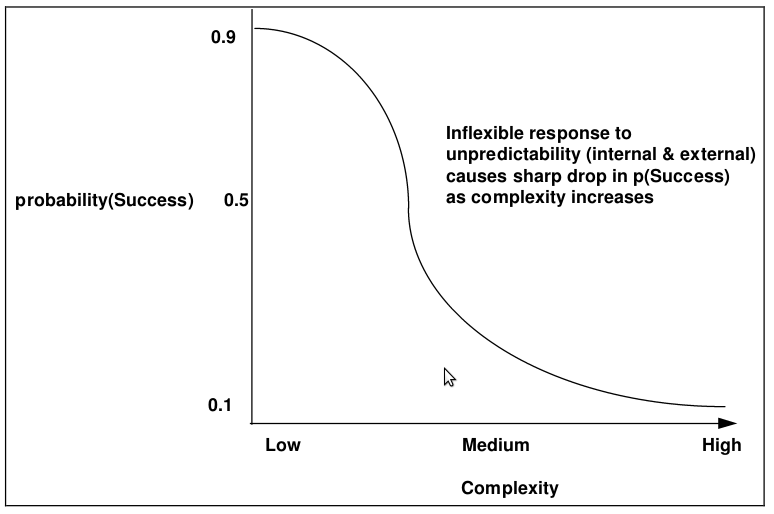
\includegraphics[width=0.5\textwidth]{scrum_risk_complexity_graph}
\caption{Gráfico Risco de Processo/Complexidade \cite{scrum_development_process}}
\label{fig:scrum_risk_complexity_graph}
\end{figure}

Considerando que o projeto da MotorBRAS deve tornar-se mais complexo à medida que requisitos forem sendo alterados (e esta alteração de requisitos é uma expectativa dos stackholders), a adoção por um modelo linear tradicional apresenta um risco, que pode ser mitigado pela adoção do Scrum. O Scrum é um processo de desenvolvimento que assume a priori que sistemas de software são complexos, de forma que flexibilidade máxima, adaptação a mudanças e controle apropriado são requeridos, pois produzir sistemas ordenados em circunstâncias complexas e caóticas exige máxima flexibilidade. \cite{scrum_development_process} 

O relacionamento entre complexidade e probabilidade de sucesso de um projeto, considerando uma metodologia flexível que incorpora controles e gerenciamento de risco, permite maior tolerância à mudanças, conforme figura que segue. 

\begin{figure}[ht!]
\centering
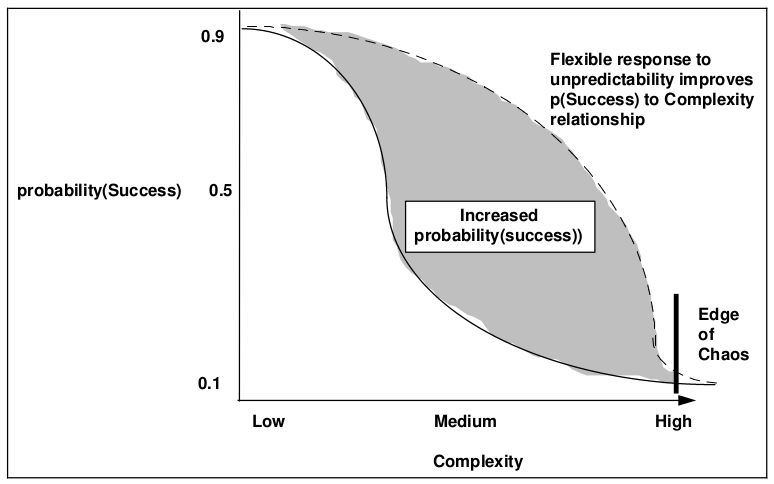
\includegraphics[width=0.5\textwidth]{scrum_risk_complexity_graph_02}
\caption{Gráfico Risco de Processo/Complexidade Com Metodologia Flexível \cite{scrum_development_process}}
\label{fig:scrum_risk_complexity_graph_02}
\end{figure}

As figuras anteriores são relativas a experiências de desenvolvimento de software em empresas como Borland, Easel, VMARK e ADM. O risco e a complexidade foram assumidos nos projetos, e projetos de sucesso foram criados. E ainda que processos ágeis ainda sejam vistos com certa ressalva, já foram provados como sendo um conjunto de métodos maduros de desenvolvimento de software. \cite{agile_meth_hype_reality}

Como forma de automação ao processo, as práticas de integração contínua e entrega contínua serão adotadas. Para a MotorBRAS, a forma pela qual a qualidade do software será medida será por meio de cobertura de código e análise estática de código. Estas métricas serão coletadas por meio de ferramentas consolidadas de mercado, capazes de gerar relatórios de acompanhamento. Além destas medidas de qualidade, a entrega de incrementos de software para teste pelos stackholders também será feita de forma automatizada, garantindo rapidez e redução de erros no processo.   

O Scrum define times de desenvolvimento dispostos entre células mutidisciplinares. Os times para o projeto MotorBRAS serão dispostos conforme segue:

\begin{itemize}
\item 1 célula de infraestrutura de comunicações: composta por 1 Product Owner, 2 analistas de requisitos, 3 programadores, 1 tester; 
\item 1 célula de customização lógica: composta por 1 Product Owner, 2 analistas de requisitos, 3 programadores, 1 tester;
\item 1 célula de customização física: composta por 1 Product Owner, 2 analistas de requisitos, 3 programadores, 1 tester;
\item 1 célula de gestão financeira e aluguel de carro: composta por 1 Product Owner, 2 analistas de requisitos, 3 programadores, 1 DBA, 1 tester;
\end{itemize}


Os analistas de requisitos precisam ter um forte entendimento do negócio e das tendências da empresa, bem como acesso livre aos stackholders. Caberá aos Analistas, juntamente com os Product Owners de cada célula, a função de interagir com os Stakeholders e definir limites e restrições necessárias para o andamento do projeto.


\subsection{Ferramentas e Métodos}

As ferramentas de modelagem de requisitos não serão formalizadas, cabendo aos desenvolvedores o acordo e a utilização de quaisquer ferramentas. Em termos de rastreabilidade e auditoria, o projeto será analisado em termos de especificações de validação automática através de testes, de forma que a modelagem dos requisitos pode, livremente, servir de apoio aos desenvolvedores, sem que precise ser formalmente controlada. A mesma filosofia vale para o design: tendo em vida o preceito ágil de que "o código é o design" \cite{fowler_design_dead}, já descrito na seção de Design deste documento, não haverá exigência por diagramas de UML. Contudo, ferramentas automatizadas de análise estática de código e cobertura de testes vão servir para validação de um código de qualidade, o que implicitamente considera uma validação de design.

O projeto fará uso da linguagem de programação Java, conforme já descrito na seção de Engenharia de Software deste documento. Além dos benefícios já citados nesta tecnologia, a Máquina Virtual Java (JVM) oferece grande poder de escalabilidade \cite{10.1109/IISWC.2005.1526008}, aspecto interessante para a MotorBRAS à medida que mais e mais carros passem a incorporar a plataforma automatizada deste projeto. Os desenvolvedores inicialmente farão uso da IDE Eclipse, da IBM, por ser a mais comumente adotada na comunidade Java \cite{java_report_2012}, reduzindo quaisquer curvas de aprendizado. Contudo, poderão substituir por outra de sua preferência (ainda visando a redução máxima com curva de aprendizado em IDE), desde que obedeça às mesmas regras de estilo de código sendo adotadas pela equipe (o código precisa seguir um mesmo padrão, independente da IDE), e que seja uma IDE consolidada no mercado, para evitar problemas que afetariam a produtividade.   

Em relação a testes, a equipe atuará em duas frentes: 
\begin{itemize}
\item em testes que validam código: pela aplicação do conceito de integração contínua \cite{ci_fowler}, que realiza a compilação do projeto e então executa testes automatizados a cada dia, notificando o time sobre divergências, assim verificando e validando a qualidade do que está sendo gravado em repositório de código
\item em testes funcionais, de caixa preta, que validam o output a partir do input: fazendo uso da ferramenta Selenium, que reproduz o uso automático da aplicação, simulando um usuário real em casos de teste previamente gravados (com base nas especificações). 
\end{itemize}

Os testes não se resumem a automatização em sua totalidade, cabendo ao engenheiro de software com perfil de tester realizar os devidos testes estruturais, exploratórios, e outros previamente descritos no tópico de testes deste documento.

Não serão adotadas ferramentas de manutenção em específico. Tendo em vista que o código está sendo produzido de forma clara (com especificações claras vinculadas a testes executáveis), não há a necessidade de utilização de ferramentas de reengenharia ou compreeensão sugeridas no SWEBOK \cite{society_software_2004}. A engenharia reversa para diagramas de classes pode ser desejável em situações de comunicação, mas por não se tratar de algo pertinente ao método de construção do software aqui proposto, não será formalizado em uma ferramenta especifica.

A gerência de configuração fará uso da ferramenta Git, por ser a que tem mais crescido no mercado \cite{scm_ranking}, além do fato de ser facilmente utilizada. Para garantia de qualidade, a ferramenta open source SonarQube será utilizada, por ser popular à comunidade Java, além de ser bastante efetiva, sendo capaz de avaliar design, arquitetura, complexidade, duplicação, regras de codificação, potenciais erros e testes \cite{quality_java_2010}.   

O método heurístico de orientação a objetos será utilizado, principalmente por caber ao problema da MotorBRAS: a necessidade do problema pode ser claramente mapeada para objetos com estado e comportamento, bem como suas interações. Além deste benefício inicial, o paradigma de orientação a objetos está diretamente vinculado à linguagem de programação Java. E conforme já descrito na seção de Requisitos deste documento, serão feitos uso de protótipos, mais especificamente para validar a necessidade do cliente em termos de requisitos.  


\subsection{Qualidade de Software}

Entende-se (e o SWEBOK \cite{society_software_2004} sugere o mesmo) que o conceito de qualidade está descrito ortogonalmente em relação a todos os tópicos anteriores deste documento. Assim, novas de‌finições faz-se-iam ambíguas, de forma que não serão aqui descritas. Contudo, alguns últimos aspectos relevantes sobre qualidade no projeto da MotorBRAS podem aqui ser mencionados:

\begin{itemize}
\item A caracterização de defeitos será utilizada conforme descrita pelo SWEBOK \cite{society_software_2004} (error, fault, failure e mistake) durante a manutenção, para gerar métricas de qualidade após a entrega do produto. O objetivo é que os stackholders do projeto da MotorBRAS possam acompanhar a qualidade do produto após a entrega e quando do produto de software em manutenção.
\item Como forma de validar a qualidade do produto imediatamente antes da entrega final, uma organização independente pode ser acionada. Esta empresa poderia dar um aval de qualidade após verificação e validação do produto de software em execução. O objetivo disto seria o de aumentar a confiança dos stackholders no produto como um todo, e entende-se ser um aspecto além da equipe de desenvolvimento do projeto, e sim uma segurança adicional a cargo dos stackholders, caso sintam necessidade. 
\end{itemize}


\section{Considerações Gerais}

O projeto aqui proposto caminha lado-a-lado com a tendência atual de preocupação com o peso da vida humana na Terra. É assumido que os governos irão cada vez mais investir em tecnologia para resolver tais problemas, ao invés de considerar que haja uma mudança drástica de consciência no ser humano de forma geral. Este projeto assume que nos próximos anos esta tendência irá se acentuar, de forma a surgir uma oportunidade no mercado que favorecerá as empresas de vanguarda. Nosso projeto caminha nesta direção. 


\section{Conclusão}

Este artigo procurou demonstrar como as diferentes disciplinas de engenharia de software expostas no SWEBOK podem ser aplicadas na resolução de um problema hipotético. A forma como as disciplinas do SWEBOK são abordadas tem um enfoque particular em práticas ágeis de desenvolvimento de software, de forma a demonstrar que tais práticas podem aplicadas dentro das orientações propostas pelo SWEBOK.

\bibliographystyle{IEEEtran}
\bibliography{eso-project}

\end{document}

